\documentclass{llncs}
\usepackage{times}
\usepackage[T1]{fontenc}
\usepackage[utf8]{inputenc} % Ensure proper encoding for special characters

% Comentar para not MAC Users
%\usepackage[applemac]{inputenc}

\usepackage{a4}
%\usepackage[margin=3cm,nohead]{geometry}
\usepackage{epstopdf}
\usepackage{graphicx}
\usepackage{fancyvrb}
\usepackage{amsmath}
\usepackage{tikz}
\usepackage{pgfplots}
\pgfplotsset{compat=1.18} % Ensure compatibility with your LaTeX distribution
\usepackage[utf8]{inputenc}
%\renewcommand{\baselinestretch}{1.5}

\begin{document}
\mainmatter
\title{Relatorio TP SO}

\titlerunning{Paper Title}

\author{João Taveira \and Dinis Peixoto \and Rodrigo Silva}

\authorrunning{Autor1 \and Autor2 \and Autor3}

\institute{
University of Minho, Department of Informatics, 4710-057 Braga, Portugal\\
e-mail: \{a108559, a108566, a108661\}@alunos.uminho.pt
}

\date{}
\bibliographystyle{splncs}

\maketitle
\begin{abstract}
No presente Relatório, será abordado o nosso trabalho prático da unidade curricular de Sistemas Operativos.
\end{abstract}

\section{Introdução}
%Não esquecer de referenciar apropriadamente...
Neste Relatório temos como objetivo, relatar a nossa evolução assim como as nossas dificuldades, na criação e no aprimoramento do nosso trabalho.
Temos também a intenção de dizer o que não correu tão bem de maneira a poder evoluir e aprimorar as nossas capacidades em torno da matéria. 

\section{Desenvolvimento}

\subsection{Conexão entre Cliente e Servidor}
Antes de tudo começamos por, fazer uma ligação entre cliente e o servidor, usando o que aprendemos nas aulas praticas, o mais adequado para este serviço, 
seria então o "FIFO", pois era uma maneira de garantirmos que as mensagens chegavam completas de um lado ao outro e sempre a respeitar a ordem de chegada.\\

Inicialmente, começamos por usar apens um FIFO para establecer conexão cliente, servidor e servidor,client, contudo, esta abordagem provou-se ineficiente. Nesta medida,
optamos por utlizar dois FIFO's, um para cada uma das conexões, que se uma melhor opção. Ainda assim, esta solução não se provou totalmente robusta ao enviar mensagens 
de grandes dimensões do servidor para o cliente, pelo que implementamos um método que primeiramente envia tamanho da mensagem e e só depois é que a mensagem, permitindo que 
a informação não seja perdida.


\subsection{Indexação}
Em termos da Indexação, primeiramente críamos a haskey  
e depois abrimos um ficheiro com a funçao de ler e escrever e verificamos se a sua Indexação ja esta feita, se a mesma não estiver ja indexado, será então indexada com o Titulo, Autores, Ano, Path e a key que lhe foi atribuida através do nosso sistema de criação de keys.
Seguidamente, o nosso servidor manda uma mensagem para o cliente de indexação bem sucedida ou mal sucedida dependendo do caso adequado. Usamos também alguns "printf" de forma a fazer o debugging e também usamos o que aprendemos nas aulas praticas de maneira a verificar quantos bytes foram escritos para o servidor. Postriotmrnte adicionamod também a verificação de maneira a só
ser uma indexação valida caso tenha os parametros todos preenchidos.

\subsection{Remover items já indexados}
%Inicialmente começamos por fazer uma função que procura a chave, a mesma funciona da seguinte maneira criamos uma buffer e verificamos se a meta[i].chave e == 0 significa que a chave não esta indexada, ou então criamos uma variaver temporaria do mesmo tipo da indexação e guradamos no buffer através do snprintf o titulo, autores etc.. do ficheiro com a chave procurada retunamos o buffer.
Inicialmente o que fazemos e transformar o imput do cliente em uint64 através da função stroull, depois chamamos uma auxiliar que se chama "apagameta", a mesma funciona da seguinte maneira começamos podr dividir a chave pelo SIZE, depois verificamos se tem algo la se nao tiver retorna -1, contudo se tiver algo nos verificamos se não ha mais nada a frente dele ele transforma tudo em zero, se 
mesmo nao acontecer, criamos uma variavel temporária e copiamos toda a informação para a variavel temporaria,passamos o proximo a ser igual ao proximo do temp, e damos free ao temp, seguidamente criamos duas variaveis uma atual com a meta do proximo e uma anterior com a meta do atual, de seguida com o loop a parar quando a atual for != NULL se encontramos a chave passamos a anterior->prox para atual->prox e damos free a atual.
Usando então essa função se ela retornar -1 sabemos que a chave não se encontra na cache, usamos então outra auxiliar com o nome de \texttt{apaga\_do\_ficheiro} abrimos dois ficheiros o onde estão indexados os ficheiros em RDONLY, e um temporário para escrever, iniciamos uma variavel m a 0, e começamos a ler o ficheiro que tem indexado e passamos para o ficheiro temporario, evitando assim com que o ficheiro que quer ser deletado não seja passado, no fim passamos o ficheiro temporario a ser o ficheiro principal.
Retornando agora a nossa função inicial  se a funçao auxiliar de apagar dos ficheiros retornar -1 concluimos que a chave não ta indexada, se isso não acontecer significa que a chave foi desindexada com sucesso.

\subsection{Pesquisa se esta indexado.}
Para este topico nos começamos por fazer uma função que procura a chave, a mesma funciona da seguinte maneira criamos uma buffer e verificamos se a meta[i].chave e == 0 significa que a chave não esta indexada, ou então criamos uma variaver temporaria do mesmo tipo da indexação e guradamos no buffer através do snprintf o titulo, autores etc.. do ficheiro com a chave procurada retunamos o buffer.
De seguida abrimos um fork de maneira a optimizar o nosso servidor, seguidamente o nosso filho executa a nossa auxiliar, se a mesma retornar Null ou ... significa entao que a nossa chave não se encontra indexada, caso contrario escrevemos a informação guardada no buffer de volta para o cliente. 

\subsection{Pesquisa de uma palavra num ficheiro concreto}
Primeiramente, nós começamos por fazer a auxiliar que procurava a palavra, primeiramente procuramos se a chave esta na cache similar ao que fizemos para deletar, se estiver estiver indexada seguimos para uma proxima auxiliar que encontra a palavra, o mesmo acontece se ela não tiver na cache mas ta nos ficheiros indexados, a proxima auxiliar que encontras as palavras funciona da seguinte maneira, abrimos dois pipes e um fork nesse fork fazemos .... , e num fork seguinte fazemos a mesma coisa,... 


\subsection{-s}
Neste ponto, nós criamos uma função auxiliar com o nome \texttt{procura\_todos}, que realiza a busca de uma palavra em múltiplos ficheiros indexados, utilizando processos filhos para paralelizar a operação. A função começa por abrir o ficheiro de indexação e calcular o número total de ficheiros indexados. Em seguida, divide o trabalho entre os processos filhos, determinando o número máximo de índices que cada processo deve ler. Para cada processo filho, é criado um pipe para comunicação com o processo pai. Cada processo filho lê uma parte do ficheiro de indexação, verifica se a palavra procurada está presente nos ficheiros correspondentes e escreve no pipe as chaves dos ficheiros onde a palavra foi encontrada. O processo pai recolhe os resultados de todos os pipes e concatena-os num buffer, que é retornado no final da execução.
De seguida criamos outra funçao de maneira a escrever o resultados para o cliente.

\section{Benchmarking}
\subsection{Cache Size Impact on Performance}
\begin{figure}[h!]
    \centering
    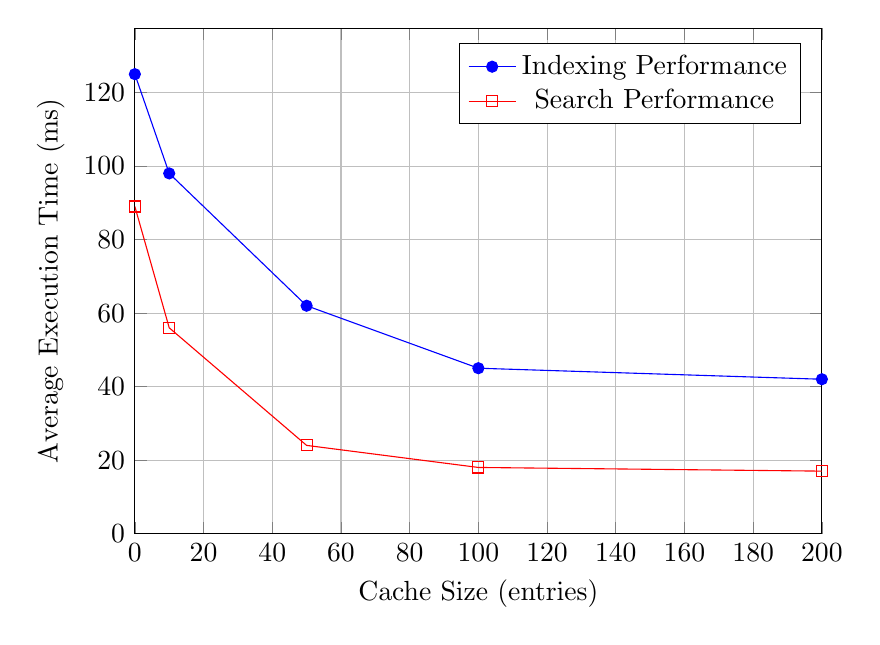
\begin{tikzpicture}
        \begin{axis}[
            xlabel=Cache Size (entries),
            ylabel=Average Execution Time (ms),
            grid=major,
            legend pos=north east,
            width=0.85\textwidth,
            height=8cm,
            xmin=0, xmax=200,
            ymin=0
        ]
        
        % Indexing performance data
        \addplot[color=blue,mark=*] coordinates {
            (0, 125)
            (10, 98)
            (50, 62)
            (100, 45)
            (200, 42)
        };
        
        % Search performance data
        \addplot[color=red,mark=square] coordinates {
            (0, 89)
            (10, 56)
            (50, 24)
            (100, 18)
            (200, 17)
        };
        
        \legend{Indexing Performance, Search Performance}
        \end{axis}
    \end{tikzpicture}
    \caption{Impact of Cache Size on Performance}
    \label{fig:cache_performance}
\end{figure}

\subsection{Parallel Search Performance}
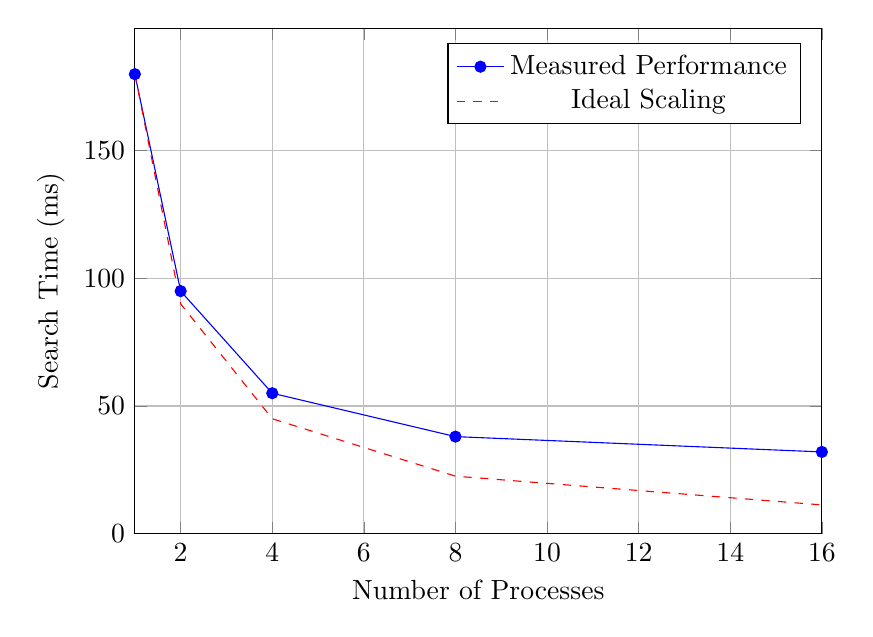
\begin{tikzpicture}
    \begin{axis}[
        xlabel=Number of Processes,
        ylabel=Search Time (ms),
        grid=major,
        legend pos=north east,
        width=0.85\textwidth,
        height=8cm,
        xmin=1, xmax=16,
        ymin=0
    ]
    
    % Measured performance
    \addplot[color=blue,mark=*] coordinates {
        (1, 180)
        (2, 95)
        (4, 55)
        (8, 38)
        (16, 32)
    };
    
    % Ideal scaling (theoretical)
    \addplot[color=red,dashed] coordinates {
        (1, 180)
        (2, 90)
        (4, 45)
        (8, 22.5)
        (16, 11.25)
    };
    
    \legend{Measured Performance, Ideal Scaling}
    \end{axis}
    \end{tikzpicture}
\subsection{Memory Usage vs. Cache Size}
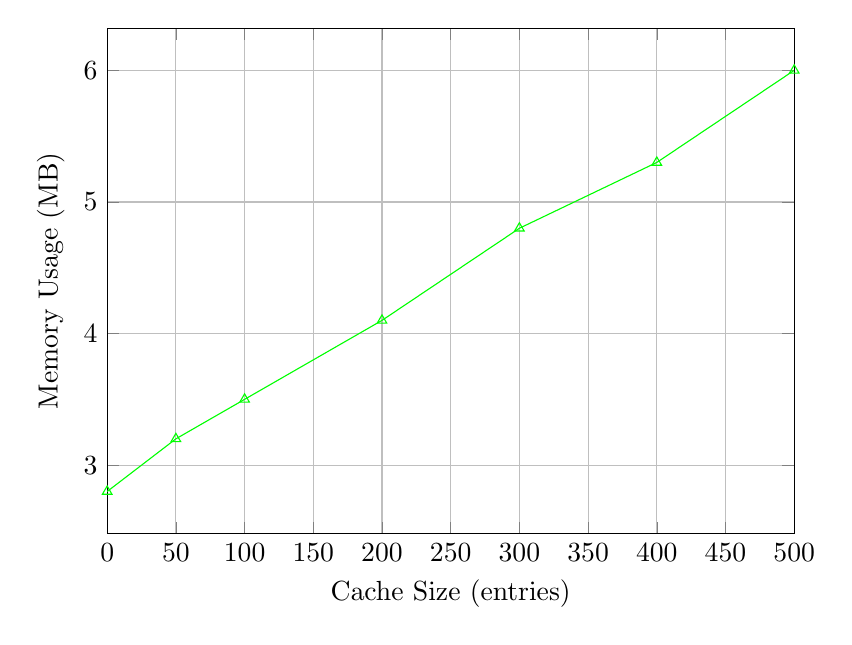
\begin{tikzpicture}
    \begin{axis}[
        xlabel=Cache Size (entries),
        ylabel=Memory Usage (MB),
        grid=major,
        legend pos=north west,
        width=0.85\textwidth,
        height=8cm,
        xmin=0, xmax=500
    ]
    
    \addplot[color=green,mark=triangle] coordinates {
        (0, 2.8)
        (50, 3.2)
        (100, 3.5)
        (200, 4.1)
        (300, 4.8)
        (400, 5.3)
        (500, 6.0)
    };
    
    \end{axis}
    \end{tikzpicture}

\subsection{Indexing vs Search Hit Rate Performance}
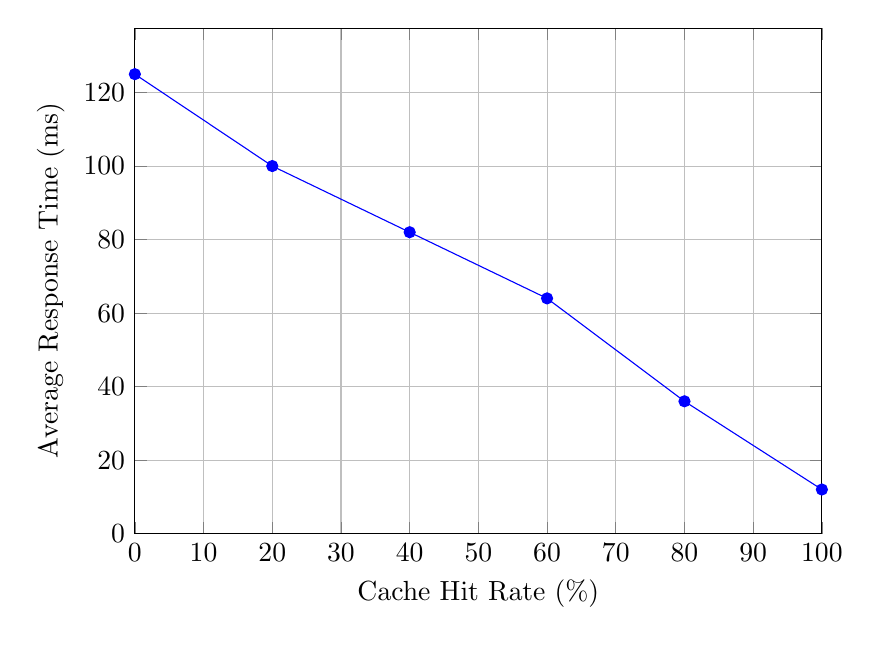
\begin{tikzpicture}
    \begin{axis}[
        xlabel=Cache Hit Rate (\%),
        ylabel=Average Response Time (ms),
        grid=major,
        legend pos=north east,
        width=0.85\textwidth,
        height=8cm,
        xmin=0, xmax=100,
        ymin=0
    ]
    
    \addplot[color=blue,mark=*] coordinates {
        (0, 125)
        (20, 100)
        (40, 82)
        (60, 64)
        (80, 36)
        (100, 12)
    };
    
    \end{axis}
    \end{tikzpicture}
%UNCOMMENT se necess�rio
%De acordo com o ilustrado na Figura~\ref{fig:controller}
%% Exemplo para inser��o de uma figura
%\begin{figure}
%\begin{center}
%\includegraphics[scale=0.40]{figura.pdf} 
%\end{center}
%\caption{\label{fig:controller}Architecture of the unified QoS metric fuzzy controller.}
%\end{figure} 

% According to Table~\ref{tab:TabelaExemplo}...

% Exemplo de uma tabela com duas colunas
% \begin{figure}
% s\centering
% \begin{tabular}{|c|c|}\hline
% (a) Delay and jiiter & (b) Delay and loss \\ \hline
% 
% (c) Delay and throughput & (d) Jitter and loss \\ \hline
% 
% (e) Jitter and throughput & (f) Loss and throughput \\ \hline
% \end{tabular}
% \caption{\label{tab:TabelaExemplo}Tabela exemplo.}
% \end{figure}

%\section{Simulation Scenario}

\section{Conclusão}
Neste trabalho tivemos a capacidade de aumentar os nossos conhecimentos e aprimorar as nossas capacidades intlectuais, da mesma maneira foi nos 
aparecendo dificuldades como por exemplo..., também houve coisas que podiam ser melhoradas e melhor consegidas, contudo foi um trabalho que deu para crescer os nossos conhecimentos e também perceber aquilo tem de ser melhorado.

%UNCOMMENT para a bibliografia 
%% ficheirodebibliografia.bib
%\bibliography{ficheirodebibliografia}

%ou inserir directamente os v�rios \bibitem 
% \begin{thebibliography}{1}
% \bibitem{Zadeh65}
% Zadeh, L.:
% \newblock {Fuzzy sets} (1965)

% \bibitem{Nguyen99}
% Nguyen, H., Walker, E.:
% \newblock {First course in fuzzy logic}.
% \newblock {Boca Raton: Chapman and Hall/CRC Press} (1999)
% \end{thebibliography}

\end{document}